%---------------------------------------------------------------------------
%	PACKAGES AND OTHER DOCUMENT CONFIGURATIONS
%---------------------------------------------------------------------------
\documentclass[final]{beamer}
\usepackage{gensymb}
\usepackage{textcomp}
\usepackage[scale=1.24]{beamerposter} % Use the beamerposter package for laying out the poster
\usetheme{confposter} % Use the confposter theme supplied with this template
\setbeamercolor{block title}{fg=Maroon,bg=white} % Colors of the block titles
\setbeamercolor{block body}{fg=black,bg=white} % Colors of the body of blocks
\setbeamercolor{block alerted title}{fg=white,bg=Maroon} % Colors of the highlighted block titles
\setbeamercolor{block alerted body}{fg=black,bg=Goldenrod!15} % Colors of the body of highlighted blocks
% Many more colors are available for use in beamerthemeconfposter.sty
%---------------------------------------------------------------------------
% Define the column widths and overall poster size
% To set effective sepwid, onecolwid and twocolwid values, first choose how many columns you want and how much separation you want between columns
% In this template, the separation width chosen is 0.024 of the paper width and a 4-column layout
% onecolwid should therefore be (1-(# of columns+1)*sepwid)/# of columns e.g. (1-(4+1)*0.024)/4 = 0.22
% Set twocolwid to be (2*onecolwid)+sepwid = 0.464
% Set threecolwid to be (3*onecolwid)+2*sepwid = 0.708
\newlength{\sepwid}
\newlength{\onecolwid}
\newlength{\twocolwid}
\newlength{\threecolwid}
\setlength{\paperwidth}{48in} % A0 width: 46.8in
\setlength{\paperheight}{38.4in} % A0 height: 33.1in
\setlength{\sepwid}{0.024\paperwidth} % Separation width (white space) between columns
\setlength{\onecolwid}{0.22\paperwidth} % Width of one column
\setlength{\twocolwid}{0.464\paperwidth} % Width of two columns
\setlength{\threecolwid}{0.708\paperwidth} % Width of three columns
\setlength{\topmargin}{-0.75in} % Reduce the top margin size
%---------------------------------------------------------------------------
\usepackage{graphicx}  % Required for including images
\usepackage{booktabs} % Top and bottom rules for tables
%---------------------------------------------------------------------------
%	TITLE SECTION 
%---------------------------------------------------------------------------
\title{Efficient heritability estimation of \\ imaging derived phenotypes} % Poster title
\author{Christian Coffman Advised by: Dr. Saonli Basu and Dr. Eric Feczko} % Author(s)
\institute{Division of Biostatistics, University of Minnesota} % Institution(s)
%----------------------------------------------------------------------------

\begin{document}
\addtobeamertemplate{headline}{} 
{\begin{tikzpicture}[remember picture,overlay] 
\node [shift={(-18cm,-9cm)}] at (current page.north east) {
\includegraphics[height=10cm]{Graphics/umn-logo.png}}; 
\end{tikzpicture}
\begin{tikzpicture}[remember picture,overlay] 
\node [shift={(-105cm,-9cm)}] at (current page.north east) {
\includegraphics[height=5cm]{Graphics/sph_logo.png}}; 
\end{tikzpicture}
}
\begin{frame}[t] % The whole poster is enclosed in one beamer frame
\begin{columns}[t] % The whole poster consists of three major columns, the second of which is split into two columns twice - the [t] option aligns each column's content to the top
\begin{column}{\sepwid}\end{column} % Empty spacer column
\begin{column}{\onecolwid} % The first column
%----------------------------------------------------------------------------
%	LEFT
%---------------------------------------------------------------------------
\begin{block}{Introduction and Objectives}

Through recent decades there has been a dramatic increase in the occurrence of behavioral health issues especially in adolescence. This has lead to a correspondingly large increase in the interest for understanding the development of the brain in adolescents. The Adolescent Brain Cognitive Development (ABCD) study is the largest long term study of the adolescent brain. Recent efforts in understanding functional connectivity focusing on graph based methods have shown different age effects throughout the brain that might be important for patterns of development in the adolescent brain. The current study focuses on evaluating the heritability of functional brain phenotypes. The large dimensionality of brain derived phenotypes requires an efficient method to estimate heritability. Here, we implement a recently development Method of Moments estaimtor (AdjHE) for heritability that dramatically increases efficiency and makes a brain wide heritability analysis feasible. 
\end{block}

\vspace{1in}

\begin{block}{Methods}
Existing MOM estimators can create severely biased heritability estimates when diverse sub populations exist. Adjusting for sub populations using PC's and other covariates. The AdjHE method has two steps:
\begin{enumerate}
    \item $y_i = C_i\gamma + \epsilon_i$, A regression on the mean level of the trait
    \item Estimate the remaining variance of the phenotype y assuming the structure of heritability remains unchanged after regressing out the mean
\end{enumerate}

\end{block}

%\begin{block}{Preprocessing}
%\begin{itemize}
%    \item Plink filter numbers 
%     \item Imputation filter settings

%\end{itemize}
%\end{block}

\vspace{1in}

\begin{alertblock}{Contact}
Email: coffm049@umn.edu \\
Github: https://github.com/coffm049
\end{alertblock}

\end{column} % End of the first column
\begin{column}{\sepwid}\end{column} % Empty spacer column
\begin{column}{\twocolwid} % Begin a column which is two columns wide (column 2)
%----------------------------------------------------------------------------
%        MIDDLE
%----------------------------------------------------------------------------
\begin{alertblock}{Heritability Estimation  Comparison}
\begin{figure}
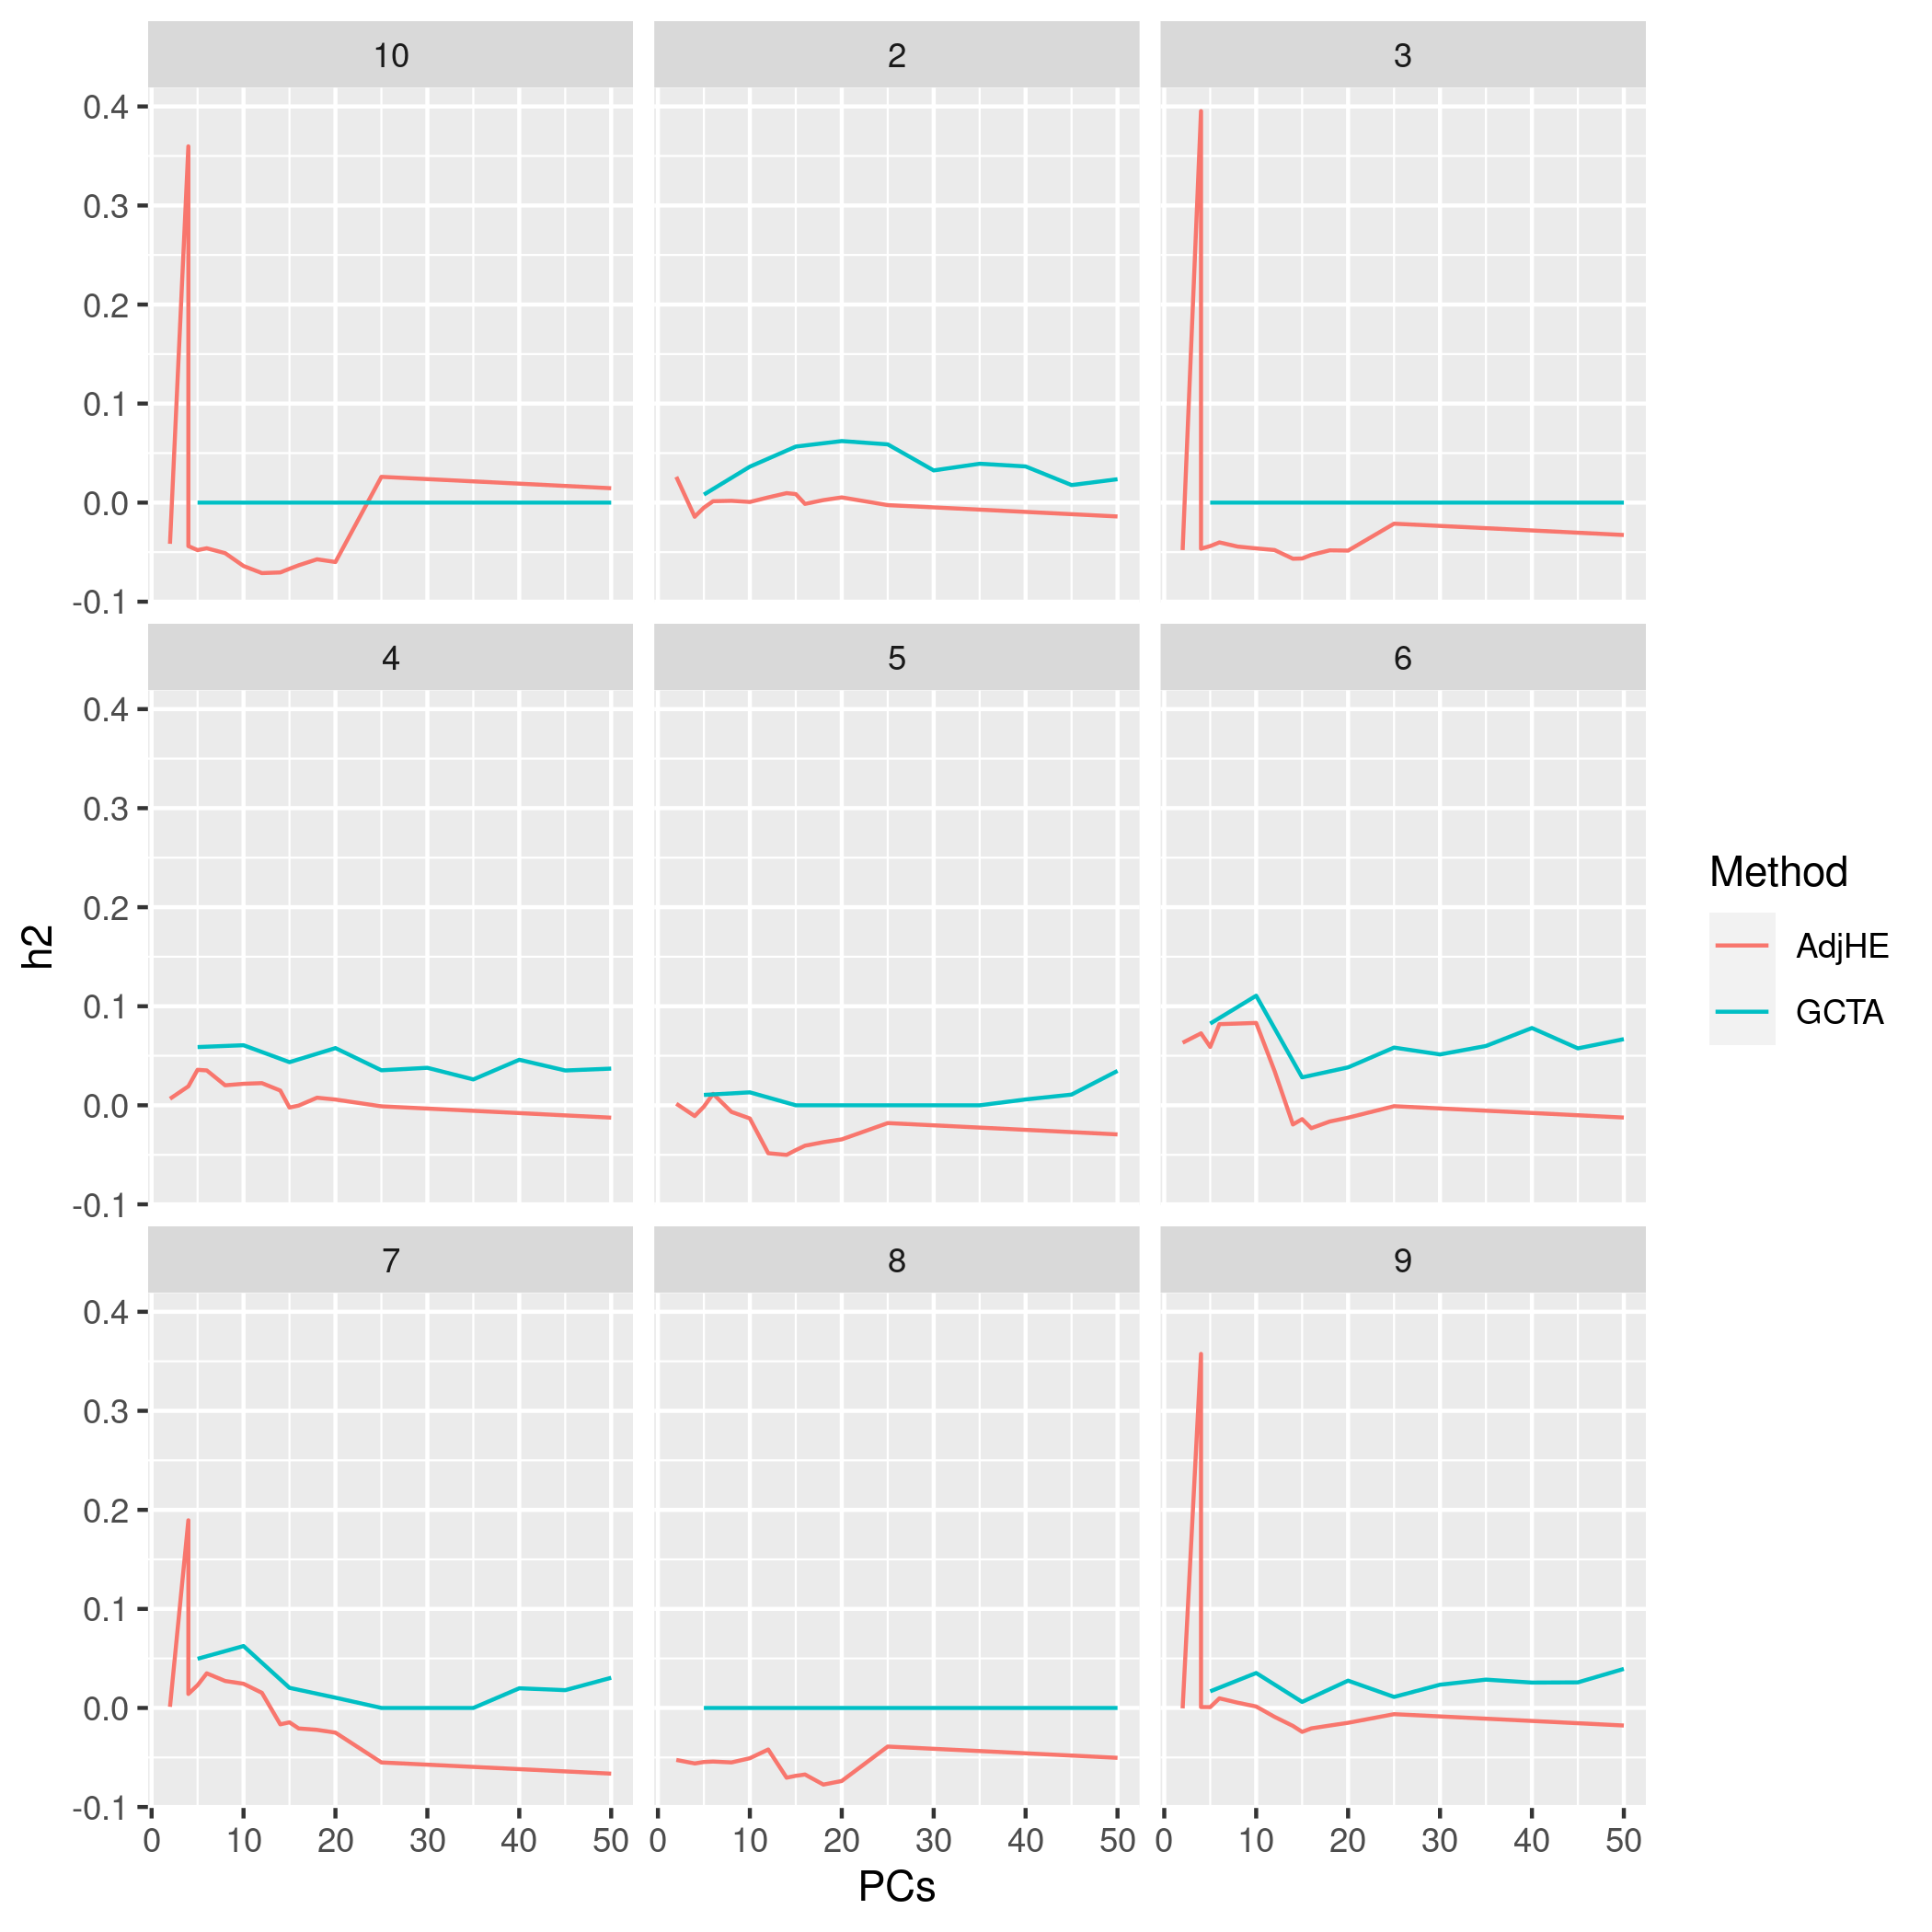
\includegraphics[width = 0.75\textwidth]{Graphics/AdjHE_GCTA_PCs.png}
\caption{Heritability estimates using GCTA and AdjHE methods controlling for differning numbers of demographic covariates (facet title) and principal components (x axes).}
\label{fig:power}
\end{figure}
\end{alertblock} 
%----------------------------------------------------------------------------
\begin{figure}
  \begin{minipage}[c]{0.67\textwidth}
    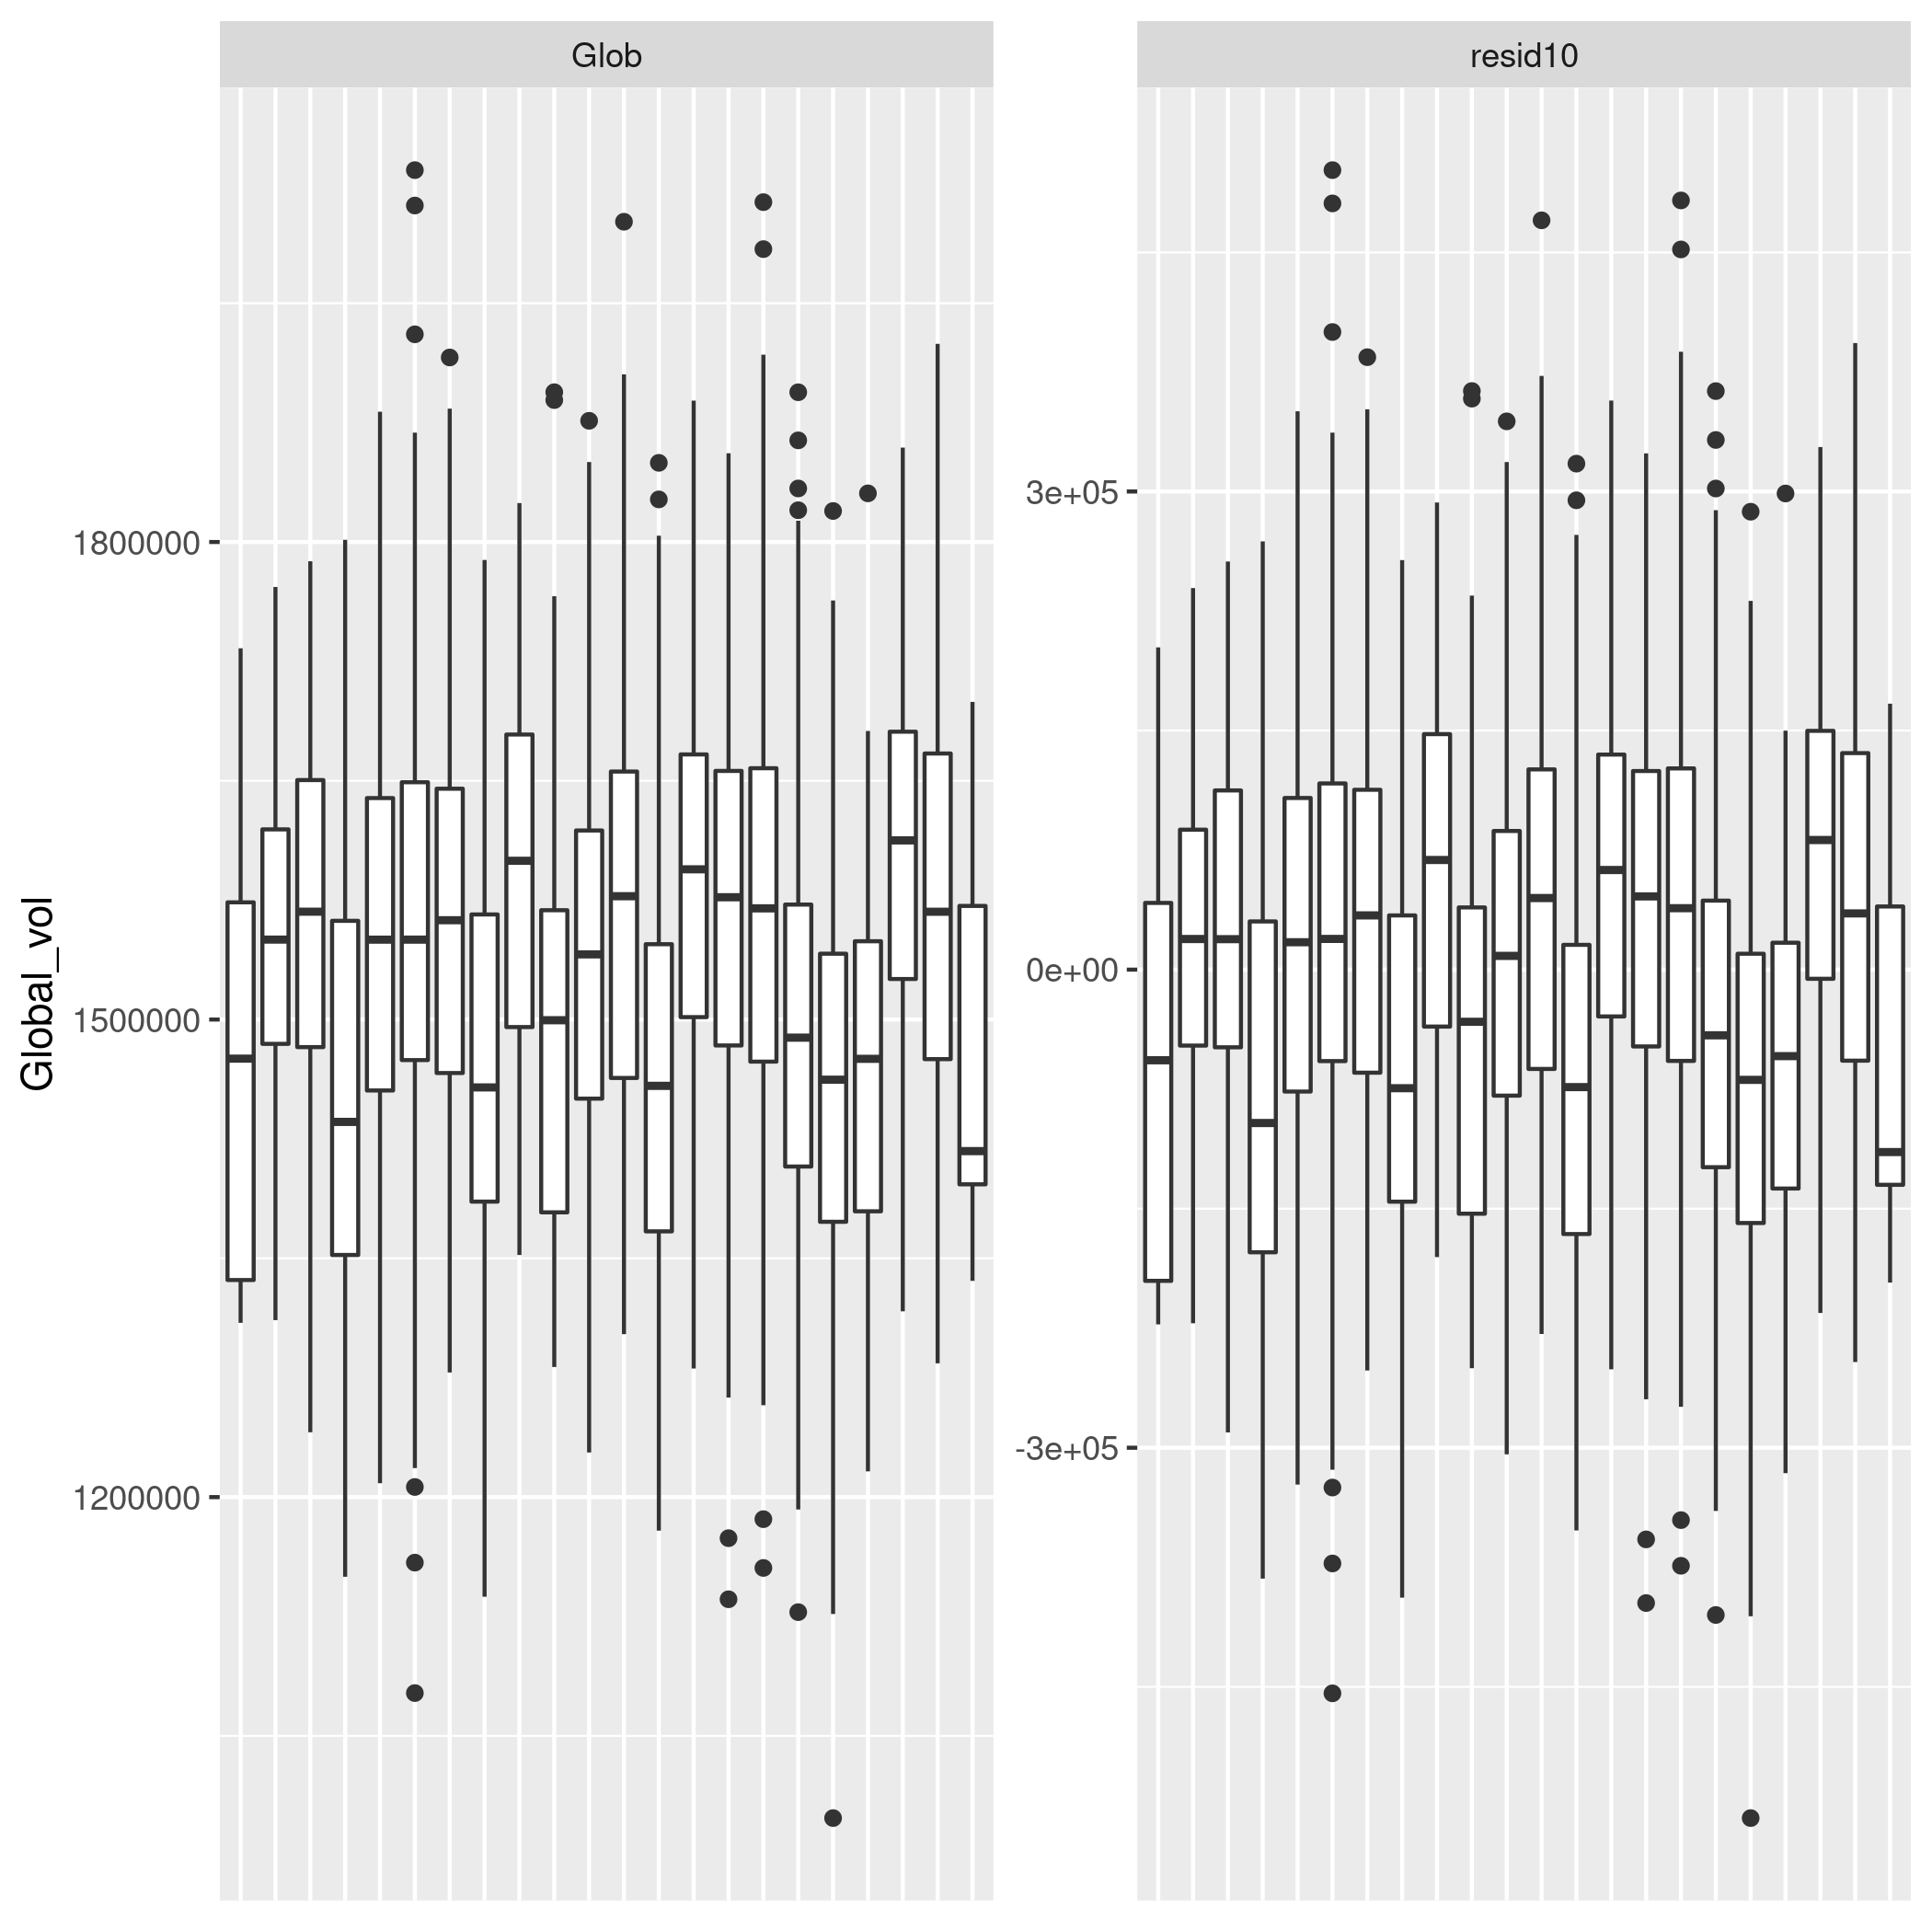
\includegraphics[width=\textwidth, height=0.6\textwidth]{Graphics/global_10pcs.png}
  \end{minipage}\hfill
  \begin{minipage}[c]{0.3\textwidth}
    \caption{\centering
       (Left) Measured global cranial volume for each of the 22 sites from the ABCD study. (Right) Residualized global cranial volume measurements after controlling for the first 10 principal genetic components.
    } \label{fig:03-03}
  \end{minipage}
\end{figure}

\end{column} % End of the second column
\begin{column}{\sepwid}\end{column} % Empty spacer column
\begin{column}{\onecolwid} % The third column
%----------------------------------------------------------------------------
%	RIGHT
%----------------------------------------------------------------------------
\begin{block}{Discussion}
Establishing a set of covariates is crucial in establishing unbiased estimates of heritability. In an effort to establish an appropriate set of covariates we've developed an efficient looping method and are looking for convergence between AdjHE estimates of heritability and the "gold-standard" for heritability estimation which is also less prone to bias when not including the best set of covariates. The imaging derived phenotypes discussed in this study are expected to have very small heritability and difficulties in identifiability between GRMs and the identity matrix necessitate a large sample size. 
\end{block}

\begin{block}{ABCD Demographics}
\begin{figure}
    \centering
    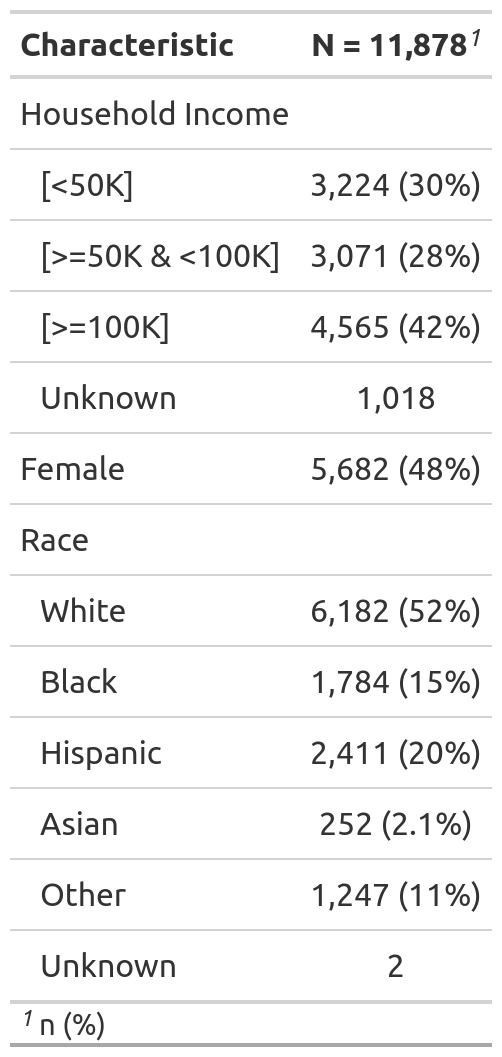
\includegraphics[width = 0.6\textwidth]{Graphics/Table1.png}
    \caption{Descriptions of key demographic variables in the ABCD dataset.
}
    \label{tab:table}
\end{figure}
\end{block}



%----------------------------------------------------------------------------
%	REFERENCES
%----------------------------------------------------------------------------
%\begin{block}{References}
%\bibliographystyle{plain}
%\bibliography{Mycoll}
%Public health assignment prompt
%\end{block}

%----------------------------------------------------------------------------
%	ACKNOWLEDGEMENTS
%----------------------------------------------------------------------------
\begin{block}{Acknowledgements}
This research was funded through a T32 grant (GM132063).
\end{block}

%----------------------------------------------------------------------------
%----------------------------------------------------------------------------


%----------------------------------------------------------------------------
\end{column} % End of the third column
\end{columns} % End of all the columns in the poster
\end{frame} % End of the enclosing frame
\end{document}